% book example for classicthesis.sty

\documentclass[a4paper,12pt]{book} % KOMA-Script book
\usepackage[UTF8,heading = true]{ctex}
\usepackage{geometry}
\geometry{a4paper,left=2cm,right=2cm,top=1.5cm,bottom=1.5cm}
\usepackage[T1]{fontenc}                
\usepackage{tikz}
\usepackage{amsthm}
\linespread{1.5}
\setlength{\parindent}{2em}
\def \_{$\rule[-6pt]{3cm}{0.05em}$}
\usepackage{pifont}
\usepackage[hidelinks]{hyperref}
\usepackage{graphicx}
\usepackage{epstopdf}
\usepackage{subfigure}
\usepackage{multirow}
\usepackage{amssymb}
\usepackage{caption}
\usepackage{ifthen}
\usepackage{verbatim}
\usepackage{circuitikz}
\usepackage{fancyhdr}%导入fancyhdr包



\usepackage{titlesec}
\pagestyle{fancy}
\fancyhead[L]{小北高中物理$\cdot$电磁感应}
\fancyhead[R]{\rightmark}
\fancyfoot[C]{\thepage}

\CTEXsetup[name={第,章},number={\chinese{chapter}}]{chapter}
\CTEXsetup[name={第,节},number={\chinese{section}}]{section}
\CTEXsetup[number={\chinese{subsection}}]{subsection}
%\CTEXsetup[name={(,)},number={\chinese{subsubsection}}]{subsubsection}
%自定义x,y轴
\newcommand\x{$x$轴}
\newcommand\y{$y$轴}
%自定义插入图片
\newcommand\pic[3]{\includegraphics[width = #1\textwidth,height = #2\textwidth]{#3}}
\newcommand\powery{++ (0,0.125) -- ++ (0,-0.25) ++ (0.125,-0.125) -- ++ (0,0.5) ++ (0,-0.25)}
\newcommand\powerx{++ (0.125,0) -- ++ (-0.25,0) ++ (-0.125,-0.125) -- ++ (0.5,0) ++ (-0.25,0)}

\newcommand\switchx{++ (2pt,0) circle (2pt) ++(2pt,0) -- ++(0.25,0.25) ++(0,-0.25)}
\newcommand\sxu[1]{++ (2pt,0) circle (2pt) ++(0,2pt) node () [above] {$#1$} ++(2pt,-2pt) -- ++(0.25,0.25) ++(0,-0.25)}
\newcommand\sxb[1]{++ (2pt,0) circle (2pt) ++(0,-2pt) node () [below] {$#1$} ++(2pt,2pt) -- ++(0.25,0.25) ++(0,-0.25)}
\newcommand\switchy{++ (0,-2pt) circle (2pt) ++(0,-2pt) -- ++(0.25,-0.25) ++(-0.25,0)}

\newcommand\Ac[1]{++ (0.25,0) circle (0.25) node () {#1} ++(0.25,0)}
\newcommand\Acy[1]{++ (0,-0.25) circle (0.25) node () {#1} ++(0,-0.25)}
\newcommand\Acs[1]{++ (0.2,-0.2) circle ({0.4*sin(45)}) node () {#1} ++(0.2,-0.2)}
\newcommand\Acss[1]{++ (0.2,0.2) circle ({0.4*sin(45)}) node () {#1} ++(0.2,0.2)}

\newcommand\R[1]{++ (0,0.125) -- ++(0,-0.25) -- ++(1,0) node () [midway,below] {$#1$} -- ++(0,0.25) -- ++(-1,0)  ++(1,-0.125)}
\newcommand\Ru[1]{++ (0,0.125) -- ++(0,-0.25) -- ++(1,0) -- ++(0,0.25) -- ++(-1,0) node () [midway,above] {$#1$} ++(1,-0.125)}
\newcommand\Ry[1]{++ (0.125,0) -- ++(-0.25,0) -- ++(0,-1) -- ++(0.25,0) -- ++(0,1) node () [midway,right] {$#1$} ++(-0.125,-1)}
\newcommand\Rb[1]{++ (0,0.125) -- ++(0,-0.25) ++(0,-0.25) -- ++(0.75,0.75) -- ++(0,-0.25) ++(0,0.25) -- ++(-0.25,0) ++(0.25,0)  ++(-0.75,-0.5) -- ++(1,0) node () [midway,below] {$#1$} -- ++(0,0.25) -- ++(-1,0)  ++(1,-0.125)}

\newcommand\SR[1]{++ (0,0.125) -- ++(0,-0.25) -- ++(1,0) -- ++(0,0.25) -- ++(-1,0)  ++ (0.5,-0.25) node () [below] {$#1$} ++(0.5,0.125) -- ++(0.125,0) -- ++(0,0.5) -- ++(-0.625,0) -- ++ (0,-0.375) -- ++(-0.125,0.125) ++(0.25,0) -- ++(-0.125,-0.125) ++(0.625,-0.125)}
\newcommand\SRy[1]{++ (0.125,0) -- ++(-0.25,0) -- ++(0,-1) -- ++(0.25,0) -- ++(0,1) node () [midway,right] {$#1$} ++(-0.125,-1) -- ++(0,-0.125) -- ++(-0.5,0) -- ++(0,0.625) -- ++(0.375,0) -- ++(-0.125,0.125) ++(0,-0.25) -- ++(0.125,0.125) ++(0.125,-0.625)}

\newcommand\bulb[1]{++(0.25,0) circle (0.25) ++({0.25*cos(45)},{0.25*sin(45)}) -- ++({-0.5*cos(45)},{-0.5*sin(45)}) ++ (0,{0.5*sin(45)}) -- ++({0.5*cos(45)},{-0.5*sin(45)}) ++ ({-0.25*cos(45)},{0.25*sin(45)}) ++ (0,-0.25) node () [below] {$#1$} ++ (0.25,0.25)}
\newcommand\bulby[1]{++(0,-0.25) circle (0.25) ++({0.25*cos(45)},{0.25*sin(45)}) -- ++({-0.5*cos(45)},{-0.5*sin(45)}) ++ (0,{0.5*sin(45)}) -- ++({0.5*cos(45)},{-0.5*sin(45)}) ++ ({-0.25*cos(45)},{0.25*sin(45)}) ++ (0.25,0) node () [right] {$#1$} ++ (-0.25,-0.25)}

\newcommand\C[1]{++ (0,0.25) -- ++(0,-0.5) ++(0.25,0) node () [below] {$#1$}-- ++(0,0.5) ++(0,-0.25)}
\newcommand\Cy[1]{++(0.25,0) -- ++(-0.5,0) ++(0,-0.25) -- ++(0.5,0) node () [right] {$#1$} ++(-0.25,0)}
\newcommand\f[1]{\fill #1 circle (2pt)}

\newcommand\rec[3]{++(0,#2/2) -- ++(0,-#2) -- ++(#1,0) -- ++(0,#2) node () [midway,right] {#3} -- ++(-#1,0)}
\newcommand\D{\Delta}
\begin{document}
\captionsetup[figure]{name={Fig.},labelsep=period,singlelinecheck=off} 
\tableofcontents  
\chapter{电磁感应}
\section{磁通量}
\subsection{磁通量定义}
\begin{itemize}
    \item 磁通量$\Phi = BS$,其中$S$为有磁场穿过的,正对磁场方向的面积,它反应了穿过线圈的磁感线的条数
    \begin{figure}[htbp]
    \centering
    \subfigure
    {
    \begin{minipage}[b]{.3\linewidth}
        \flushleft
        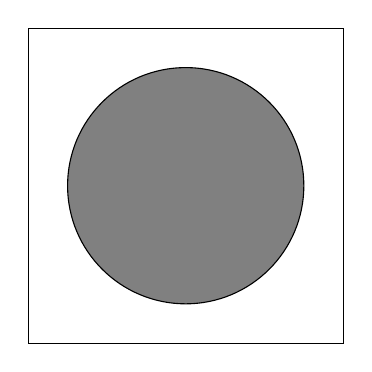
\begin{tikzpicture}
            \fill [color = gray] (0,0) circle (1.5);
            \draw (0,0) circle (1.5);
            \draw (-2,-2) -- (2,-2) -- (2,2) -- (-2,2) -- cycle;
        \end{tikzpicture}
    \end{minipage}
    }
    \subfigure
    {
    \begin{minipage}[b]{.3\linewidth}
        \flushleft
        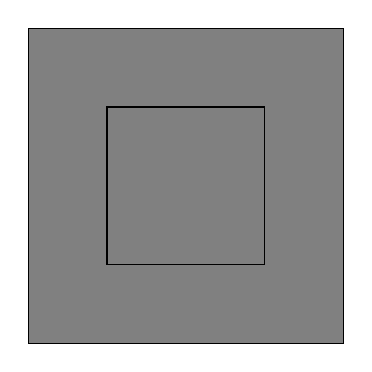
\begin{tikzpicture}
            \fill [color = gray] (0,0) -- (4,0) -- (4,4) -- (0,4) -- cycle;
            \draw (0,0) -- (4,0) -- (4,4) -- (0,4) -- cycle;
            \draw (1,1) -- (3,1) -- (3,3) -- (1,3) -- cycle;
        \end{tikzpicture}
    \end{minipage}
    }
    \subfigure
    {
    \begin{minipage}[b]{.3\linewidth}
        \flushleft
        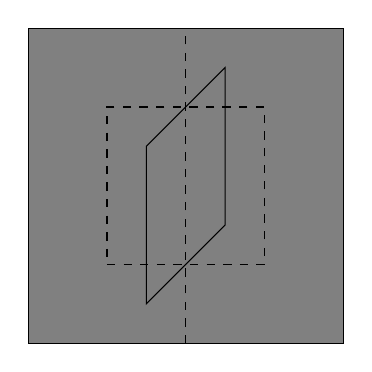
\begin{tikzpicture}
            \fill [color = gray] (0,0) -- (4,0) -- (4,4) -- (0,4) -- cycle;
            \draw (0,0) -- (4,0) -- (4,4) -- (0,4) -- cycle;
            \draw[dashed] (1,1) -- (3,1) -- (3,3) -- (1,3) -- cycle;
            \draw[dashed] (2,0) -- (2,4);
            \draw (1.5,2.5) -- (2.5,3.5) -- (2.5,1.5) -- (1.5,0.5) -- cycle;
        \end{tikzpicture}
    \end{minipage}
    }
\end{figure}
    \item 严格来说$\Phi = BS$cos$\theta$,$\theta$是磁场与线圈的夹角,但我们不知道夹角如何计算,因此我们会定义线圈的某一个面为正面,另一个面为反面,磁场从正面穿入时,磁通量为正,反之则为负
    \item 一个$N$匝,面积为$S$的线圈,放入磁感应强度为$B$的磁场中,则通过线圈的磁通量为\_
    \item 磁通量是标量,因此正负磁通量可以直接计算抵消
    \begin{figure}[htbp]
        \centering
        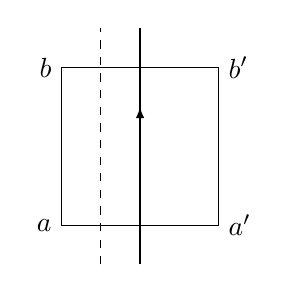
\begin{tikzpicture}
            \draw[-latex] (0,0) -- (0,2);
            \draw (0,1.5) -- (0,3);
            \draw (-1,0.5) node () [left] {$a$} -- (-1,2.5) node () [left] {$b$} -- (1,2.5) node () [right] {$b^\prime$} -- (1,0.5) node () [right] {$a^\prime$} -- cycle;
            \draw [dashed] (-0.5,0) -- (-0.5,3);
        \end{tikzpicture}
    \end{figure}
\end{itemize}

\subsection{磁通量与感应电流}
当穿过\textbf{闭合线圈}的磁通量发生\textbf{变化}时,便会产生感应电流
\newpage
\subsection{例题}
1.如图所示,框架面积为$S$,框架平面与磁感应强度为B的匀强磁场方向垂直,则下列穿过平面的磁通量的说法中不正确的是()\par
\begin{figure}[htbp]
    \centering
    \begin{tikzpicture}
        \draw (-2,0) -- (2,0) -- (2,2) -- (-2,2) --cycle;
        \draw[dashed] (0,-1) node () [right] {$O^\prime$} -- (0,3) node () [right] {$O$};
        \foreach \i in {-3,...,3}{
            \foreach \j in {-1,...,3}{
                \node at (\i,\j) {$\times$};
            }
        }
    \end{tikzpicture}
\end{figure}
A.在如图所示位置时磁通量大小等于BS\par
B.若使框架绕$OO^\prime$转过60$^\circ$角,磁通量大小为$\frac{1}{2}$BS\par
C.若从初始位置转过 90$^\circ$角,磁通量大小为BS\par
D.若从初始位置转过 180$^\circ$角,磁通量变化量的大小为2BS\\

2.如图所示,在条形磁铁外套有A,B两个同心的,大小不同的圆环,穿过 A 环的磁通量$\Phi_A$与穿过B 环的磁通量$\Phi_B$相比较,有()\par
A.$\Phi_A < \Phi_B\qquad$
B.$\Phi_A = \Phi_B\qquad$
C.$\Phi_A > \Phi_B\qquad$
D.不能确定\\

3.下列四幅图能产生感应电流的是()\par
\begin{figure}[htbp]
    \centering
    \subfigure
    {
    \begin{minipage}[b]{.4\linewidth}
        \flushleft
        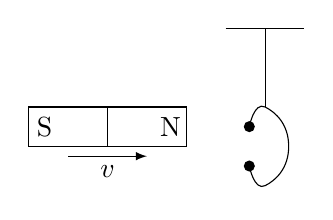
\begin{tikzpicture}
            \draw (0,0) -- (2,0) -- (2,0.5) -- (0,0.5) -- cycle;
            \draw (1,0) -- (1,0.5);
            \node at (0.2,0.25) {S};
            \node at (1.8,0.25) {N};
            \draw[-latex] (0.5,-0.125) -- ++(1,0) node () [midway,below] {$v$};
            \draw (2.5,1.5) -- ++(1,0);
            \draw (3,1.5) -- ++(0,-1);
            \draw plot [smooth,tension = 1] coordinates{
                (2.8,0.25) (3,0.5) (3.3,0) (3,-0.5) (2.8,-0.25)
            };
            \fill (2.8,0.25) circle (2pt);
            \fill (2.8,-0.25) circle (2pt);
        \end{tikzpicture}
        \caption*{A}
    \end{minipage}
    }
    \subfigure
    {
    \begin{minipage}[b]{.4\linewidth}
        \flushleft
        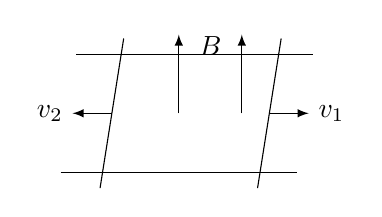
\begin{tikzpicture}
            \draw (0,0) -- (3,0);
            \draw (0.2,1.5) -- ++(3,0);
            \draw (0.5,-0.2) -- (0.8,1.7);
            \draw [-latex] (0.65,0.75) --++(-0.5,0) node () [left] {$v_2$};
            \draw (2.5,-0.2) -- (2.8,1.7);
            \draw [-latex] (2.65,0.75) -- ++(0.5,0) node () [right] {$v_1$};
            \draw[-latex] (1.5,0.75) -- ++(0,1);
            \draw[-latex] (2.3,0.75) -- ++(0,1);
            \node at (1.9,1.6) {$B$};
        \end{tikzpicture}
        \caption*{B}
    \end{minipage}
    }
    
    \subfigure
    {
    \begin{minipage}[b]{.4\linewidth}
        \flushleft
        \begin{tikzpicture}
            \draw (0,0) ellipse (1 and 0.5);
            \draw[dashed] (-1.5,0) --  ++(3,0);
            \draw[dashed] (0,0) -- (0,0.75);
            \draw[-latex] (-1,0.75) -- (0,0.75);
            \draw (-0.25,0.75) -- ++(1,0);
            \node at (0,1) {通入增大的电流};
        \end{tikzpicture}
        \caption*{C}
    \end{minipage}
    }
    \subfigure
    {
    \begin{minipage}[b]{.4\linewidth}
        \flushleft
        \begin{tikzpicture}
            \draw (0,0) -- (1,0) -- (1,0.5) -- (0,0.5) -- cycle;
            \draw[-latex] (1,0.25) -- ++(0.5,0) node () [above] {$v$};
            \foreach \i in {-1,...,2}{
                \foreach \j in {-1,...,1}{
                    \node at (\i,\j) {$\times$};
                }
            }
        \end{tikzpicture}
        \caption*{D}
    \end{minipage}
    }
\end{figure}

\subsection{磁场与线圈的夹角(选)}
事实上,通过数学的立体几何板块的学习,我们是可以求出磁场与线圈的夹角的,这个角上是线圈的法向量与磁场的夹角,而法向量是任意垂直于线圈,且从\textbf{固定的某一面}穿出线圈的向量,这个面也就是所谓的线圈正面

\newpage
\section{楞次定律}
\end{document}


